% Template latex non officiel pour rapport de TP EEA.
% C'est un template pour thèse que j'ai adapté et 
% auquel j'ai ajouté des éléments au fil du temps pour mes rapports de TP.
% En cas de problèmes n'hésites pas a me contacter.
% David Tocaven
% david.tocaven@gmail.com


%%% /!\ /!\ /!\ /!\ /!\ /!\
% Se compile avec PDFLatex
%%% /!\ /!\ /!\ /!\ /!\ /!\
%%=================================================%%
%%						MAIN
%%=================================================%%


\documentclass[a4paper]{report}

%====================== PACKAGES ======================
\usepackage{bbold}
\usepackage{soul}				% souligner
\usepackage{dsfont}
\usepackage[french]{babel}		% Pour avoir le document en français
\usepackage[utf8]{inputenc}	% Encodage du document
\usepackage{float}				% Pour gérer les positionnement d'images
\usepackage{amsmath}
\usepackage{mathrsfs}			% Pour les lettres calligraphiques équation
\usepackage[colorinlistoftodos]{todonotes}
\usepackage{url}				% Pour faire des hyperliens vers le web
\usepackage{color}
% pour les informations sur un document compilé en PDF et les liens externes / internes
\usepackage{hyperref}			% Pour faire des hyperliens
\usepackage{array}				% Pour faire des tableaux
\usepackage{tabularx}
% pour utiliser 		% floatbarrier
\usepackage{placeins}
%\usepackage{floatrow}
\usepackage{setspace}			% Espacement entre les lignes
	\usepackage{abstract}			% Modifier la mise en page de l'abstract
\usepackage[T1]{fontenc}		% Police et mise en page (marges) du document
\usepackage[top=2cm, bottom=2cm, left=2cm, right=2cm]{geometry}
\usepackage{pdfpages}			% pour inclures des pdf comme des images
\usepackage{subfig}				% Pour les galerie d'images
\usepackage{listings}			% pour inclure du code dans le doc
\usepackage{soul}				% Pour surligner
\usepackage{enumitem}

\sethlcolor{grisclair}
\definecolor{darkgreen}{RGB}{0,100,0}


%====================== INFORMATION ET REGLES ======================

%rajouter les numérotation pour les \paragraphe et \subparagraphe
\setcounter{secnumdepth}{4}
\setcounter{tocdepth}{4}

\hypersetup{							% Information sur le document
pdfauthor = { NOM },				% Auteurs
pdftitle = {Matière - Titre - Sujet },		% Titre du document
pdfsubject = {matière},		% Sujet
pdfkeywords = {},				% Mots-clefs
pdfstartview={FitH}}					% ajuste la page à la largueur de l'écran
%pdfcreator = {MikTeX},% Logiciel qui a crée le document
%pdfproducer = {}} % Société avec produit le logiciel

\newcounter{cpt1}						% Compteur pour les n° de ligne dans les prog de l'annexe1
\newcommand\increm{\arabic{cpt1}\addtocounter{cpt1}{1}}
%initialisation de l'intégrateur de language C



%======================== DEBUT DU DOCUMENT ========================

\begin{document}

%\lstset{
%  language=C,                	  % choose the language of the code
%  numbers=left,                   % where to put the line-numbers
%  stepnumber=1,                   % the step between two line-numbers.
%  numbersep=5pt,                  % how far the line-numbers are from the code
%  backgroundcolor=\color{white},  % choose the background color. You must add \usepackage{color}
%  showspaces=false,               % show spaces adding particular underscores
%  showstringspaces=false,         % underline spaces within strings
%  showtabs=false,                 % show tabs within strings adding particular underscores
%  tabsize=2,                      % sets default tabsize to 2 spaces
%  captionpos=b,                   % sets the caption-position to bottom
%  breaklines=true,                % sets automatic line breaking
%  breakatwhitespace=true,         % sets if automatic breaks should only happen at whitespace
%  title=\lstname,                 % show the filename of files included with \lstinputlisting;
%}
%régler l'espacement entre les lignes
\newcommand{\HRule}{\rule{\linewidth}{0.5mm}}


%page de garde
%%=================================================%%
%%						TITRE DU DOCUMENT (1 PAGE)
%							  Pas totalement fini
%%=================================================%%

\begin{titlepage}
\begin{center}

% Upper part of the page. The '~' is needed because only works if a paragraph has started.


\includegraphics[width=0.60\textwidth]{./page_de_garde/logo_ups.png}~\\[1cm]

\textsc{\LARGE Université Paul Sabatier}\\[1.5cm]

\textsc{\Large \bf Diagnostic et Supervision }\\[0.5cm]

% Title
\HRule \\[0.4cm]

{\huge \bfseries  - Rapport de Travaux Pratiques :\\ \textsc{BE : Commande Supervisée} -}

\HRule \\[1.5cm]

% Author and supervisor
\begin{minipage}{0.4\textwidth}
\begin{flushleft} \large
\emph{Auteurs: }\\
%Prenom \textsc{Nom}\\
David \textsc{TOCAVEN}\\
Lucien \textsc{RAKOTOMALALA}\\
\end{flushleft}
\end{minipage}
\begin{minipage}{0.58\textwidth}
\begin{flushright} \large
\emph{Encadrant:} \\
\textbf{Euriell \textsc{LE CORRONC}}
\end{flushright}
\end{minipage}
\newline
\newline

% une éventuelle image
%\includegraphics[width=.6\textwidth]{./page_de_garde/BACDO_schema.pdf}~\\[1cm]

\vfill
% logo fsi & eea
\begin{tabular}{cc}
   
\includegraphics[height=2cm]{./page_de_garde/logo_fsi.png} \hspace{2cm} &
    \hspace{2cm}
   
\includegraphics[height=2cm]{./page_de_garde/logo_eea.jpg} \\
\end{tabular}

% Bottom of the page
{\large \today}

\end{center}
\end{titlepage}
	

%page blanche
\newpage
~
\tableofcontents
\thispagestyle{empty}
\setcounter{page}{0}
%ne pas numéroter le sommaire


%espacement entre les lignes d'un tableau
\renewcommand{\arraystretch}{1.5}

%====================== INCLUSION DES PARTIES ======================
%
%~
\thispagestyle{empty}
%recommencer la numérotation des pages à "1"
\setcounter{page}{0}

\chapter*{Introduction}
\addcontentsline{toc}{chapter}{Introduction}
\label{chap:Intro}
Nous avons réalisé ce Travaux pratiques dans le cadre du module Autonomie de notre Master 2 ISTR. Nous avons pu pendant ce TP mettre en oeuvre le cours de Commande par Supervision sur 3 exemples de systèmes : un système de maintenance automatisé, un atelier de peinture et de polissage et enfin sur un protocole de communication. 

Ces 3 systèmes vont faire appel à nos compétences de modélisation de procédé et de compréhension de spécifications. Nous utiliserons par la suite le logiciel DESUMA pour tout calcul de produit parallèle ou produit synchrone entre automate ainsi que certain algorithme de ce même logiciel pour obtenir les propriétés des commande supervisée que nous obtiendrons.	% Importation de introduction.tex

\chapter{Système de Maintenance automatisé}
Le 1er modèle est un système contenant deux machines $M_1$ et $M_2$ dont la maintenance doit être assurée car celles-ci peuvent tomber en pannes. Pour représenter notre système à commander, nous avons pris comme représentation de  $M_1$ et $M_2$ les automates :
\begin{center}
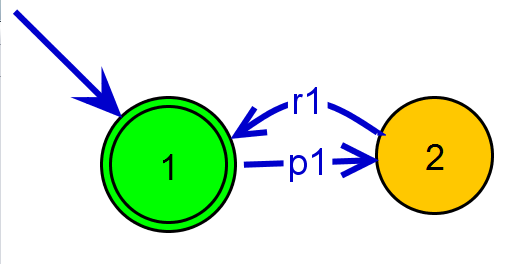
\includegraphics[scale=0.3]{I/images/M1.png}
\captionof{figure}{Machine $M_1$}
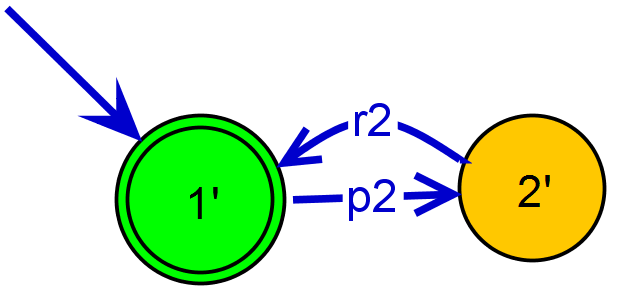
\includegraphics[scale=0.3]{I/images/M2.png}
\captionof{figure}{Machine $M_2$}
\end{center}
où : \begin{itemize}[label = \textbullet]
\item $p_1$ et $p_2$ sont les pannes sur les machines $M_1$ et $M_2$.
\item $r_1$ et $r_2$ sont les réparations sur les machines $M_1$ et $M_2$.
\end{itemize}


Nous avons obtenu le modèle $P$, soit le produit parallèle entre $M_1$ et $M_2$ (EXPLICATION) suivant à l'aide de DESUMA : 
\begin{center}
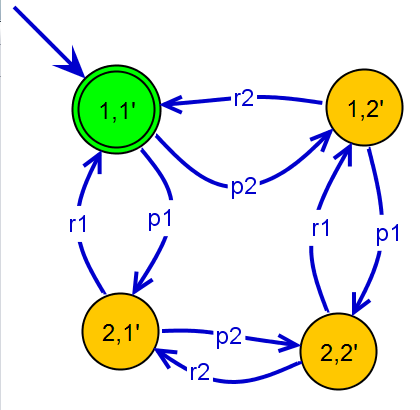
\includegraphics[scale=0.5]{I/images/P.png}
\captionof{figure}{Modèle automate $P$}
\end{center}
Nous utilisons le produit parallèle pour obtenir un automate qui laisse toutes les possibilités d'évolution à $M_1$ et $M_2$. Or, le système complet $P$, en supposant que $M_1$ et $M_2$ sont indépendants, permet de présenter toutes les évolutions de $M_1$ et de $M_2$ tel que : $P = \Sigma(M_1)\ U\ \Sigma(M_1)$.

Nous obtenons le modèle des spécifications $S_1$ suivant :\\
\begin{center}
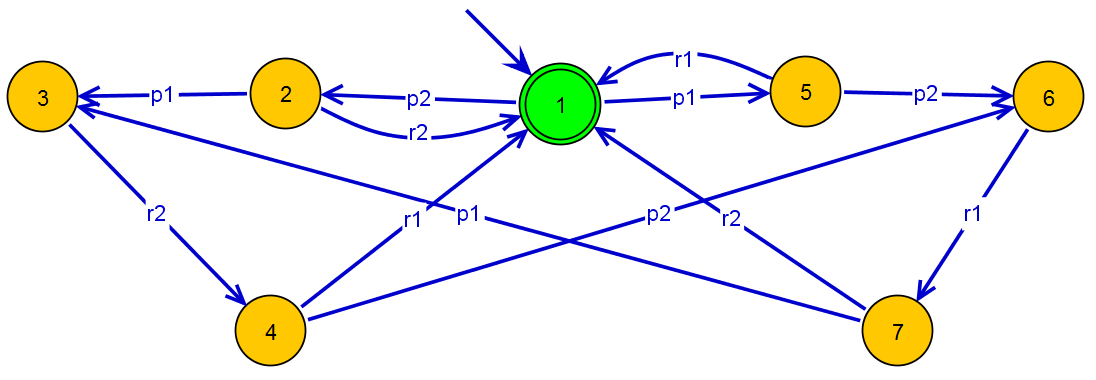
\includegraphics[scale=0.5]{I//images/S1.png}
\captionof{figure}{Modèle automate $S$}
\end{center}dans lequel nous relevons les propriétés suivantes :
\begin{itemize}[label = \textbullet]
\item Spécification totale car les langages de $S_1$ et de $P$ sont identiques : $\Sigma_{S_1} = \Sigma_P$
\item Spécification dynamique car notre automate $S_1$ représente les séquences d'évènements autorisées.
\end{itemize}

Notre modèle de spécifications nous amène donc à la commande supervisé suivante :\begin{center}

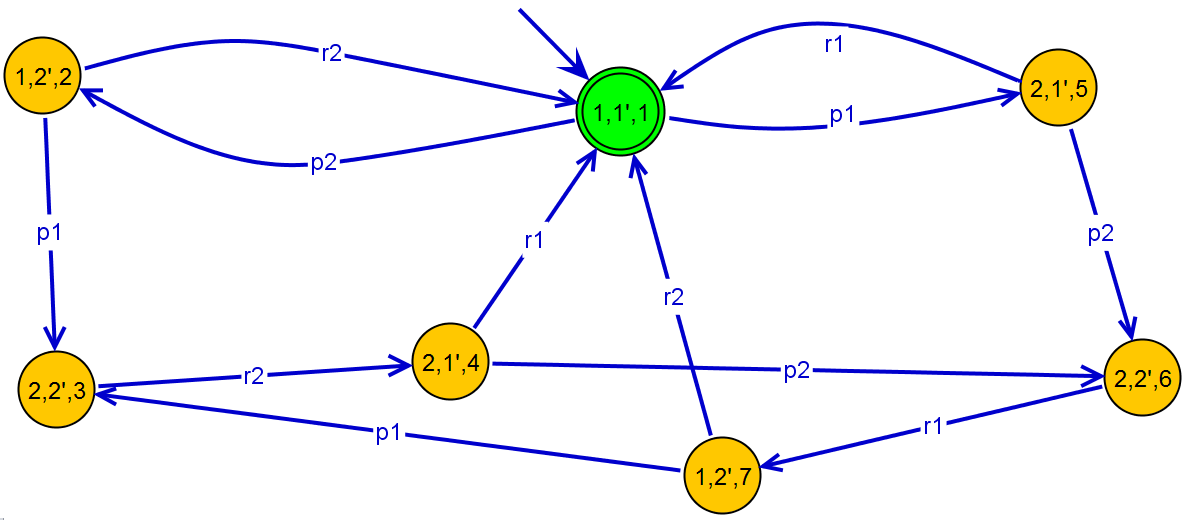
\includegraphics[scale=0.3]{I/images/P_S1.png}
\captionof{figure}{Modèle de commande supervisé $P/S_1$}

\end{center}construit à l'aide du produit parallèle car la spécification est partielle.
A l'aide de DESUMA, nous avons pu vérifier la propriété de commandabilité de notre automate de commande supervisé, nous sommes donc capable d'affirmer qu'aucun évènements non contrôlable ne va causer des séquences non définis par $S_1$.
\begin{center}
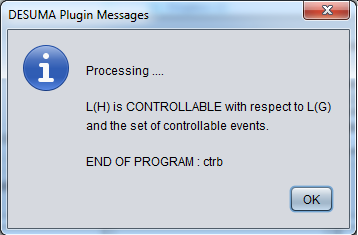
\includegraphics[scale=0.5]{I/images/P_S1_ctrbl.png}
\captionof{figure}{Message DESUMA}
\end{center}
Pour vérifier le non blocage de notre commande supervisé, nous allons vérifier que chaque état de $P/S_1$ est co-accessible, ce qui revient à déterminer si chaque état peut accéder à l'état marqué. Ce état est la paire (1,1), et nous constatons que touts les autres paire $(x_P,x_S)$ ont accès via une séquence la paire d'états marqués. La commande obtenue est donc non bloquante ce qui conclut notre première étude de cas. 

\chapter{Atelier de peinture et de polissage}
Passons maintenant à un système composé d'un atelier et d'un robot qui permet de réaliser les actions peinture/polissage pour ensuite déservir les pièces dans un stock. Pour la modélisation des automates At (atelier) et St (stock), nous avons choisi les modèles suivants :
\begin{figure}[!ht]
\begin{minipage}{.5\textwidth}
\centering
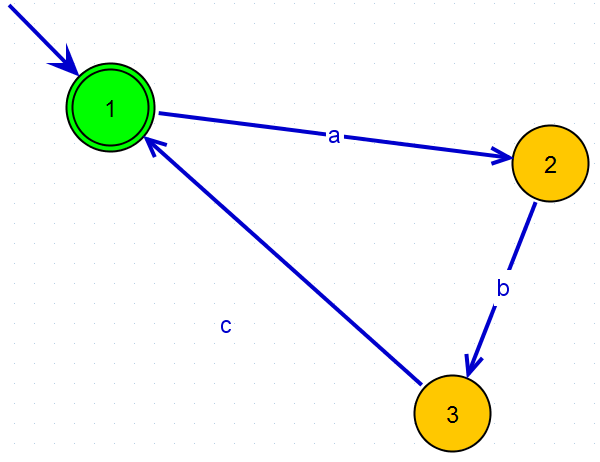
\includegraphics[width=\textwidth]{./II/images/At.png}
\caption{Atelier At}
\end{minipage} \hfill
\begin{minipage}{.5\textwidth}
\centering
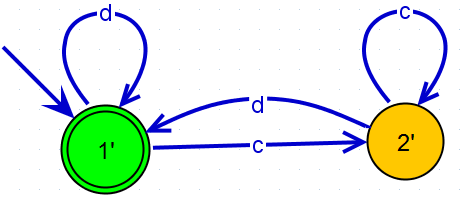
\includegraphics[width=\textwidth]{./II/images/St.png}
\caption{Stock St}
\end{minipage}
\end{figure}

avec pour alphabet de At et St:
\begin{itemize}[label = \textbullet]
\item $\Sigma_{At} = \left\lbrace a,b,c \right\rbrace $
\item $\Sigma_{St} = \left\lbrace c,d\right\rbrace$
\item les évènements non contrôlables sont : $\Sigma_{nc}=\left\lbrace b,c \right\rbrace$, tous les autres évènements sont observables et contrôlables.
\end{itemize}

En utilisant le produit parallèle, nous avons obtenu notre modèle du procédé qui est le suivant : \begin{figure}
\centering
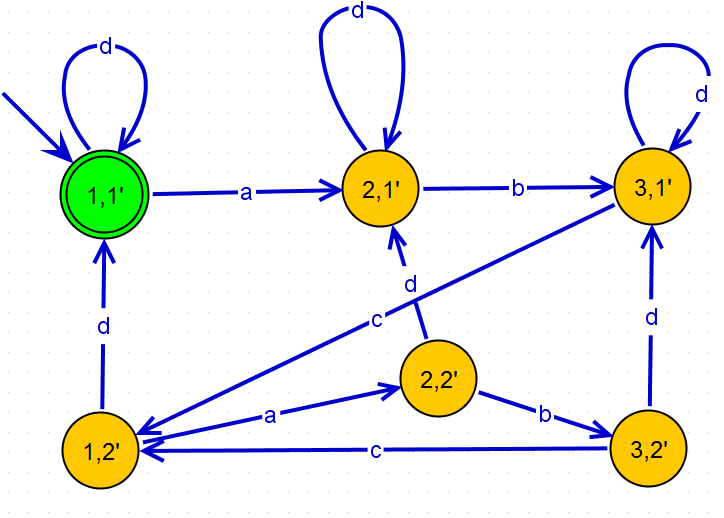
\includegraphics[width = 0.5\textwidth]{./II/images/P.png}
\caption{Modèle de procédé}
\end{figure}

En suivant les consignes de l'objectif, nous avons modélisé notre modèle de spécifications cette manière, \begin{figure}[!ht]
\centering
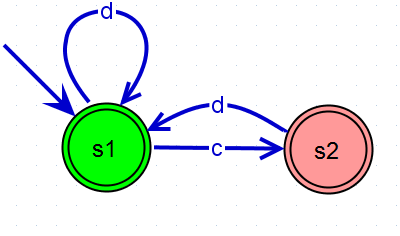
\includegraphics[width = 0.5\textwidth]{./II/images/S.png}
\caption{Modèle des spécifications}
\end{figure}
représenté sur $\Sigma_S = \left\lbrace c,d\right\rbrace$. Nous remarquons que l'ensemble des évènements est strictement inclus dans l'ensemble $\Sigma_{P_o}$, ensemble des évènements observables de $P$, donc notre spécifications est dite partielle. Nous avons de même une représentation de séquence d'évènements autorisées donc notre spécification est dite dynamique.

Notre commande supervisé obtenu avec DESUMA est (produit parallèle):\begin{figure}[!ht]
\centering
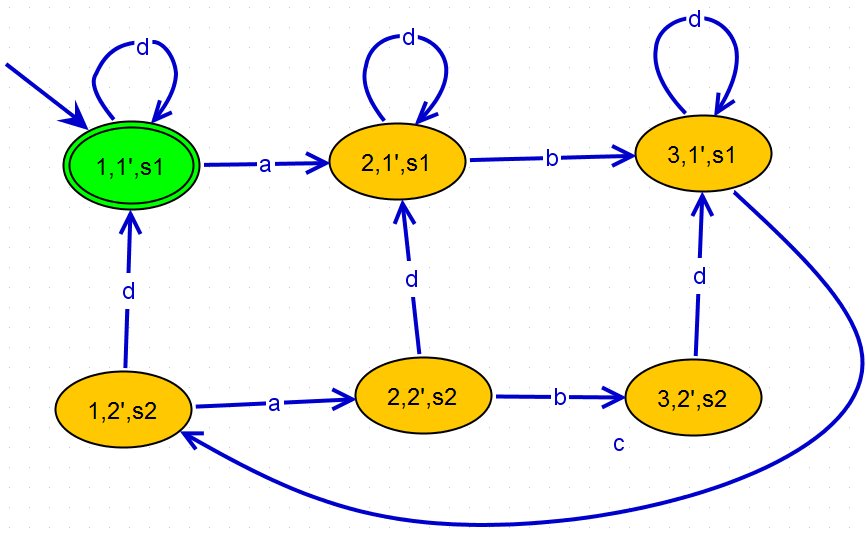
\includegraphics[width = 0.5\textwidth]{./II/images/P_S.png}
\caption{Modèle de commande supervisé}
\end{figure}

L'analyse de DESUMA nous indique que notre modèle n'est pas contrôlable. En effet,  partir de l'état $(3,2)$, il est possible d'avoir une séquence contenant $c$, qui n'est pas contrôlable, qui cause une séquence non souhaitée par les spécifications. C'est pourquoi nous allons maintenant utiliser un algorithme pour rendre P/S contrôlable comme vu pendant nos cours de Diagnostic et Supervision. L'exécution de celui ci est détaillé ci dessous :
\begin{itemize}[label = \textbullet]
\item Nous commençons avec $Q = 0$ et $Q'=0$
\item Vérifions que chaque état ($x_P$,$x_S$) ne contient pas de transition $\delta_S(x_S,\sigma_{nc})\not\in X_S$ et $\delta_P(x_P,\sigma_{nc})\in X_P$ avec $\sigma_{nc}\in\Sigma_{P/S}$ : \\C'est le cas pour la paire ($x_{P_3}$,$x_{S_2}$), on l'ajoute alors à $Q$ : $Q = \left\lbrace (x_{P_3},x_{S_2}) \right\rbrace $
\item Vérifions maintenant qu'aucune séquence non contrôlable de peut amener à une des paires de $Q$ :\\
$\exists s_{nc}$ / $\delta*(x_{P_2},x_{S_2}) \in Q$, alors $Q' = Q\ U\ \left\lbrace x_{P_3},x_{S_2}\right\rbrace$
\item Finalement, nous obtenons : $X_{P/S} = X_{P/S} \backslash \left\lbrace (x_{P_3},x_{S_2}),(x_{P_2},x_{S_2}) \right\rbrace$.
\end{itemize}
\newpage
En enlevant les deux paires (3,2) et (2,2), nous permettons à notre commande supervisé d'être contrôlable. En utilisant cette conclusion, nous obtenons notre commande supervisé contrôlable décrite par le modèle de gauche. Il est cependant possible d'utiliser l'outil de $Controlability$ de DESUMA pour calculer cet automate. Nous le décrivons sur la figure de droite.\begin{figure}[!ht]
\begin{minipage}{.5\textwidth}
\centering
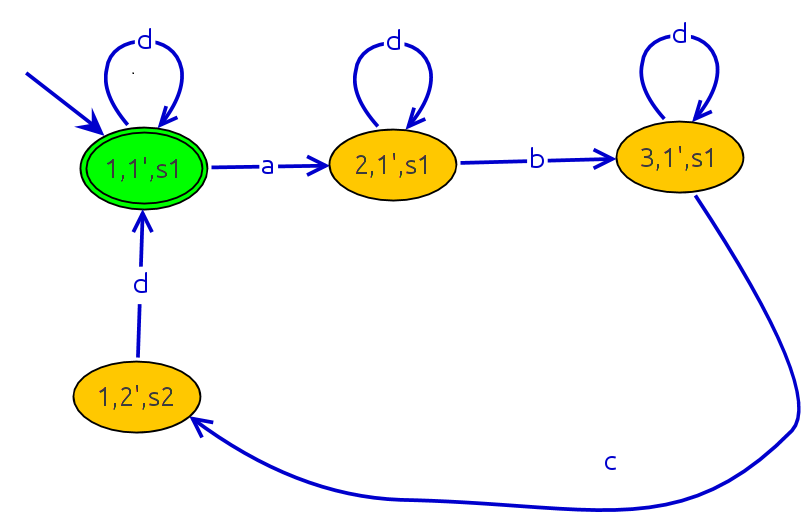
\includegraphics[width=\textwidth]{./II/images/P_S_automate_ctrb_manuel.png}
\caption{Bouchon}
\end{minipage} \hfill
\begin{minipage}{.5\textwidth}
\centering
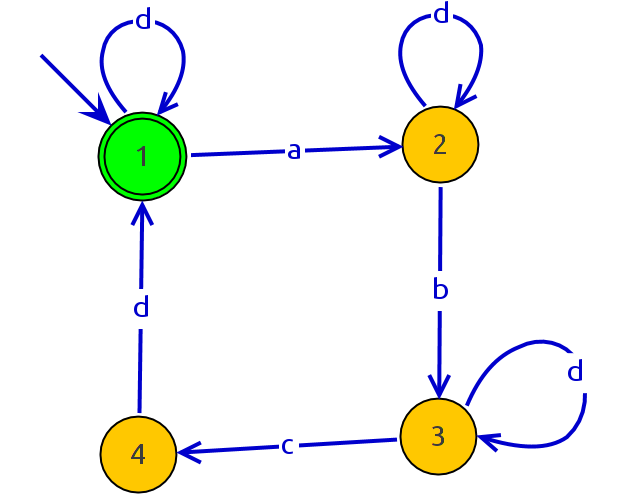
\includegraphics[width=\textwidth]{./II/images/P_S_automate_ctrb_desuma.png}
\caption{Bouteille}
\end{minipage}
\end{figure}


Cependant, cette propriété ne garantit pas le non blocage de notre nouvel automate. A partir de l'état marqué $(1,1')$, nous remarquons que pour chaque état il existe une séquence permettant d'accéder à l'état marqué. Notre commande supervisé est co-accessible et donc non bloquante.

\chapter{Protocole de communication informatique}
Nous considérons maintenant un système de communication informatique mis en place entre un client et deux serveurs, un serveur principal et un autre de secours utilisé quand le premier tombe en panne. Le but du système est de permettre au client de pouvoir envoyer deux types de messages : $m_1$ et $m_2$  l'aide de l'un des deux serveur.

Nous avons alors choisi de représenter le modèle du procédé de ce système par l'automate suivant :
\begin{figure}[!ht]
\begin{minipage}{0.5\textwidth}
\centering
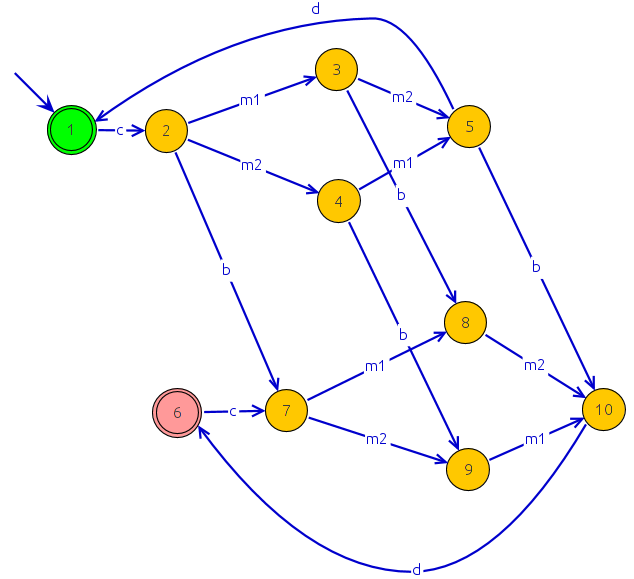
\includegraphics[width = \textwidth]{./III/images/P.png}
\caption{Modèle de procédé}
\end{minipage}
\begin{minipage}{0.5\textwidth}
Avec : \begin{itemize}[label = \textbullet]
\item $\Sigma_P = \left\lbrace m_1, m_2, b, c, d \right\rbrace$
\item $\Sigma_O =  \left\lbrace m_1, m_2, b, c, d \right\rbrace$
\end{itemize}
\end{minipage}
\end{figure}
Soit avec la particularité suivante : une fois que le serveur est tombé en panne, celui ci nécessite une dépannage manuel et donc l'automate serait ré-intialisé. 

Les spécifications de notre système sont que chaque l'émission des messages vers le serveur doivent respectés l'ordre $m_1 \rightarrow m_2$, nous obtenons l'automate 
\begin{center}
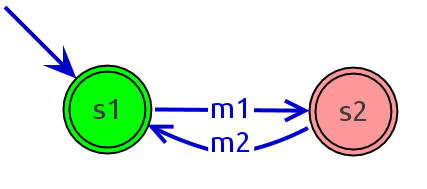
\includegraphics[width = .5\textwidth]{./III/images/S.png}
\captionof{figure}{Modèle des spécifications}
\end{center}
Nous pouvons maintenant calculé avec un produit parallèle et DESUMA la commande supervisé que nous allons appliquer. Nous seront aptes par la suite à déterminer les propriétés de notre commande. L'automate est :\begin{figure}[!ht]
\begin{minipage}{.5\textwidth}
\centering
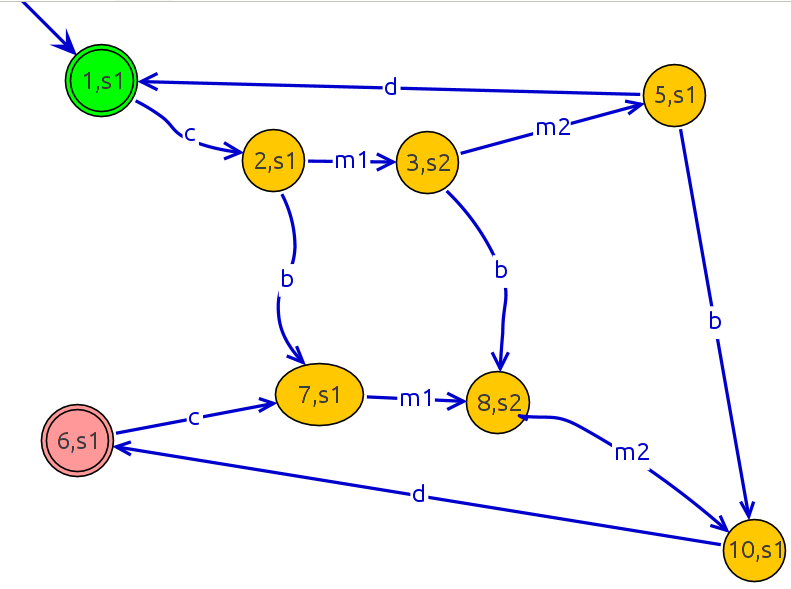
\includegraphics[width=\textwidth]{./III/images/P_S.png}
\caption{Modèle de commande supervisée}
\end{minipage} \hfill
\begin{minipage}{.5\textwidth}
\centering
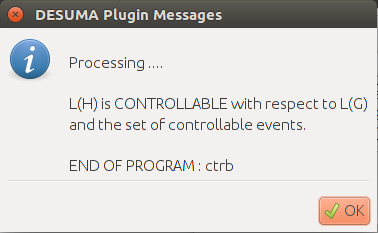
\includegraphics[width=\textwidth]{./III/images/P_S_ctrbl.png}
\caption{Message DESUMA sur la contrôlabilité}
\end{minipage}
\end{figure}

L'algorithme de vérification de DESUMA n'a pas trouvé de séquence d'évènements non contrôlable ne respectant pas $S$, notre commande est donc contrôlable. Les états marqués $(1,s1)$ et $(6,s1)$ sont accessibles par n'importe quel état, la commande est donc non-blocante.

%\chapter{}



%\input{./V/chap5.tex}

%\input{./VI/chap6.tex}

%\input{./conclusions/conclusions.tex}

%\chapter{Conclusion}

% %Ne pas numéroter cette partie
\part*{Annexes}
%Rajouter la ligne "Annexes" dans le sommaire
\addcontentsline{toc}{part}{Annexes}

\chapter*{Annexe 1 - TITRE}
\addcontentsline{toc}{chapter}{TITRE}
%\setcounter{section}{0}
% **********************************
\addcontentsline{toc}{section}{TITRE}
\label{Annex:NOM_FICHIER}
\lstset{
  language=Matlab,                	  % choose the language of the code
  basicstyle=\ttfamily,
  numbers=left,                   % where to put the line-numbers
  stepnumber=1,                   % the step between two line-numbers.
  numbersep=5pt,                  % how far the line-numbers are from the code
  backgroundcolor=\color{white},  % choose the background color. You must add \usepackage{color}
  commentstyle = \color{darkgreen},
  showspaces=false,               % show spaces adding particular underscores
  showstringspaces=false,         % underline spaces within strings
  showtabs=false,                 % show tabs within strings adding particular underscores
  tabsize=2,                      % sets default tabsize to 2 spaces
  captionpos=b,                   % sets the caption-position to bottom
  breaklines=true,                % sets automatic line breaking
  breakatwhitespace=true,         % sets if automatic breaks should only happen at whitespace
  %caption=exo1.m,                 % show the filename of files included with \lstinputlisting;
  literate={á}{{\'a}}1 {è}{{\`e}}1 {é}{{\'e}}1,
}
%\lstinputlisting{./annexes/annexe1/NOMFICHIER.m} %{language = MAtlab}
\chapter*{Annexe 2 - TITRE}
\addcontentsline{toc}{chapter}{Annexe 2 - TITRE}
\setcounter{section}{0}
\setcounter{subsection}{0}
% **********************************
	%


\newpage

%récupérer les citation avec "/footnotemark"
\nocite{*}

%%choix du style de la biblio
%\bibliographystyle{unsrt}
%%inclusion de la biblio
%\bibliography{bibliographie}
%%voir wiki pour plus d'information sur la syntaxe des entrées d'une bibliographie

\end{document}

